\subsubsection{Testbench và Kết quả mô phỏng ALU}

\textbf{a. Mô tả kịch bản kiểm chứng (Testbench)} \\
Môi trường mô phỏng (Testbench) được xây dựng nhằm kiểm tra toàn diện chức năng của khối số học và logic (ALU). Kịch bản kiểm tra (stimulus) được thiết kế với các mục tiêu cụ thể:
\begin{itemize}
    \item \textbf{Quét toàn bộ tập lệnh:} Lần lượt cấp các tín hiệu \texttt{opcode} từ \texttt{000} đến \texttt{111} kết hợp với các giá trị \texttt{inA} và \texttt{inB} khác nhau để kiểm tra ngõ ra \texttt{out}.
    \item \textbf{Kiểm tra tính bất đồng bộ của \texttt{is\_zero}:} Thử nghiệm thay đổi \texttt{inA} đột ngột để quan sát sự phản hồi ngay lập tức của cờ \texttt{is\_zero} mà không cần phụ thuộc vào xung clock hay sự thay đổi của \texttt{opcode}.
    \item \textbf{Bẫy lỗi (Corner Case):} Tạo test case số 9 thực hiện phép cộng số bù 2: $10 + (-10)$. Kết quả phép tính bằng 0 nhưng toán hạng \texttt{inA} $\neq 0$. Mục tiêu là chứng minh cờ \texttt{is\_zero} chỉ phụ thuộc vào \texttt{inA} theo đúng đặc tả của lệnh nhảy \texttt{SKZ}.
\end{itemize}

\textbf{b. Mã nguồn Testbench (Verilog)}
\begin{lstlisting}[language=Verilog, caption={Mã nguồn Testbench kiểm tra khối ALU}, label={lst:tb_alu}]
`timescale 1ns / 1ps

module tb_ALU();

    
    reg  [31:0] inA;
    reg  [31:0] inB;
    reg  [2:0]  opcode;
    
    wire [31:0] out;
    wire        is_zero;

    
    localparam HLT = 3'b000, SKZ = 3'b001, ADD = 3'b010, AND = 3'b011,
               XOR = 3'b100, LDA = 3'b101, STO = 3'b110, JMP = 3'b111;

    
    ALU uut (
        .inA(inA),
        .inB(inB),
        .opcode(opcode),
        .out(out),
        .is_zero(is_zero)
    );

   
    initial begin
       
$display("--------");
        $display("Time|Opcode|inA(hex)|inB(hex)|out(hex)|is_zero");
        $display("-------");
        
       
        $monitor("%8t|%b|%h|%h|%h|%b", 
                 $time, opcode, inA, inB, out, is_zero);

        
        inA = 32'd0; 
        inB = 32'd0; 
        opcode = HLT;
        #10; 
        
        // TEST CASE 1:  ADD 
       
        inA = 32'd15; 
        inB = 32'd25; 
        opcode = ADD;
        #10; 

       
        // TEST CASE 2:  AND 
        
        inA = 32'hFFFF0000; 
        inB = 32'hFF00FF00; 
        opcode = AND;
        #10; 

        
        // TEST CASE 3: XOR
        
        inA = 32'hAAAAAAAA; 
        inB = 32'h55555555; 
        opcode = XOR;
        #10; 

       
        // TEST CASE 4:  LDA (Load inB)
       
        inA = 32'd99; 
        inB = 32'h1234ABCD; 
        opcode = LDA;
        #10; 

       
        // TEST CASE 5:  inA (HLT, SKZ, STO, JMP)
       
        inA = 32'hCAFEBA5E; 
        inB = 32'd0; 
        opcode = STO;
        #10; 

      
        // TEST CASE 6:  is_zero 
       
        inA = 32'd0; 
        inB = 32'd999; 
        opcode = ADD;
        #10; 

      
        // TEST CASE 7:  SKZ with inA = 0
      
        inA = 32'd0; 
        inB = 32'hFFFFFFFF; 
        opcode = SKZ;
        #10; 

        
        // TEST CASE 8: is_zero nhay su thay doi inA ko thay doi opcode
      
        inA = 32'd5;
        #5;  
        inA = 32'd0;
        #5;  
        
        
        // TEST CASE 9: inA != 0 but result=0
inA = 32'd10;
inB = -32'd10; 
opcode = ADD;
#10;


        $display("-----------");
        $display("HOAN THANH MO PHONG!");
        $finish; 
    end

endmodule

\end{lstlisting}

\textbf{c. Sơ đồ mạch RTL (RTL Schematic)} \\
Quá trình tổng hợp (Synthesis) từ mã nguồn Verilog đã tạo ra sơ đồ mạch logic của ALU. Sơ đồ cho thấy bộ dồn kênh (Multiplexer) được tối ưu hóa để định tuyến dữ liệu dựa trên tín hiệu \texttt{opcode}, và một bộ dò cờ Zero (Zero Flag Detector) được kết nối trực tiếp vào bus \texttt{inA}.

\begin{figure}[H]
    \centering
    % Hãy thay 'alu_rtl_schematic.png' bằng ảnh sơ đồ mạch ALU xuất ra từ phần mềm (Vivado/Quartus)
    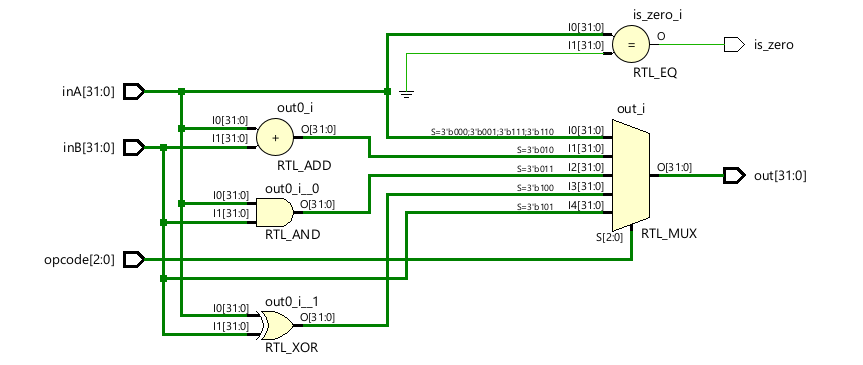
\includegraphics[width=0.85\textwidth]{machALU.png} 
    \caption{Sơ đồ mạch logic (RTL Schematic) của khối ALU}
    \label{fig:alu_rtl}
\end{figure}

\textbf{d. Kết quả xuất ra màn hình (Console Output)} \\
Thông qua các hàm hệ thống \texttt{\$monitor} và \texttt{\$display}, toàn bộ sự kiện thay đổi tín hiệu được ghi nhận lại theo thời gian thực.

\begin{figure}[H]
    \centering
    % Hãy thay 'alu_console.png' bằng ảnh chụp màn hình terminal Vivado của bạn
    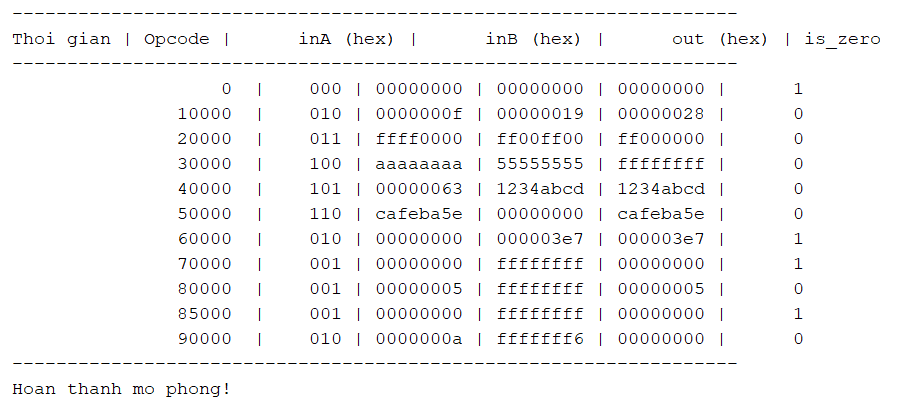
\includegraphics[width=0.75\textwidth]{cosoleALU.png} 
    \caption{Kết quả chạy Testbench khối ALU hiển thị trên Console}
    \label{fig:alu_console}
\end{figure}

Dựa vào bảng kết quả trên Console, các phép toán \texttt{ADD}, \texttt{AND}, \texttt{XOR} và các lệnh nạp dữ liệu hoạt động hoàn toàn chính xác. Tại thời điểm 90000 ps, phép toán \texttt{10 + (-10)} cho ra \texttt{out = 00000000} nhưng \texttt{is\_zero = 0} (vì \texttt{inA = 0000000a}), minh chứng thiết kế đã đúng tính chất bất đồng bộ .

\textbf{e. Giản đồ sóng (Waveform)} \\
Giản đồ thời gian cung cấp cái nhìn trực quan nhất về sự thay đổi của các tín hiệu điện. 

\begin{figure}[H]
    \centering
    % Hãy thay 'alu_waveform.png' bằng ảnh chụp giản đồ sóng của bạn
    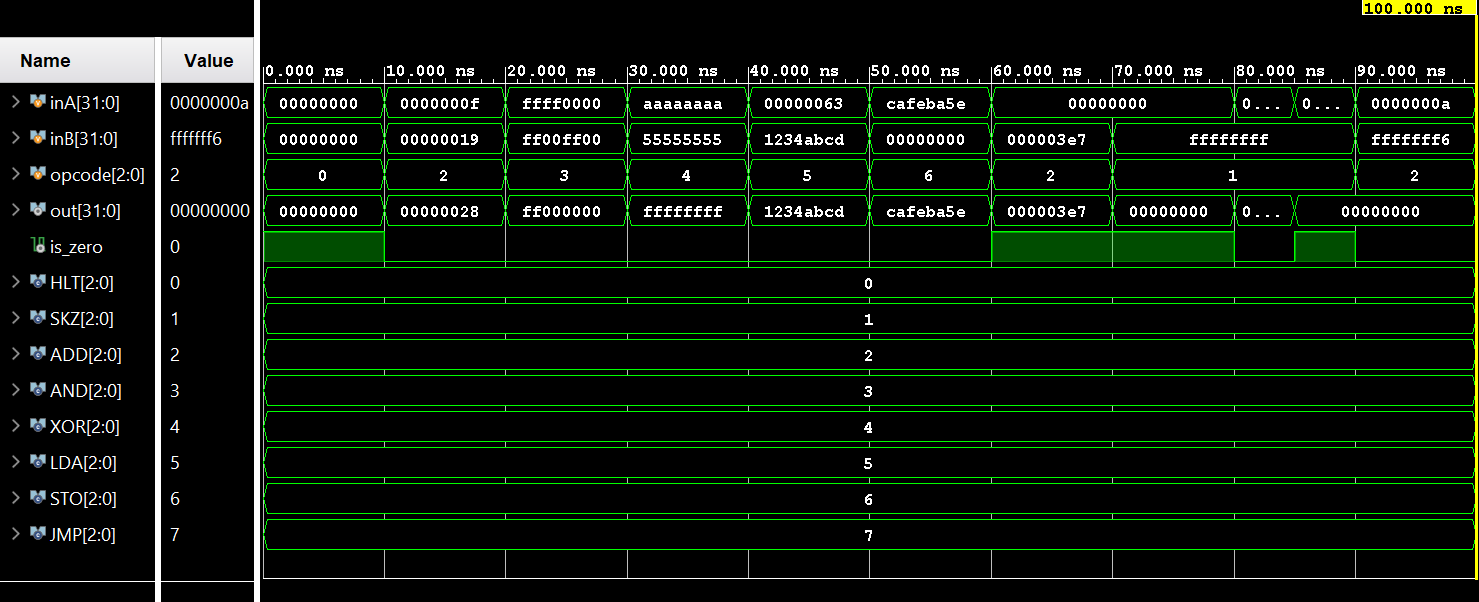
\includegraphics[width=\textwidth]{waveALU.png} 
    \caption{Giản đồ thời gian (Waveform) minh họa hoạt động của ALU}
    \label{fig:alu_waveform}
\end{figure}

Trên giản đồ sóng, có thể dễ dàng nhận thấy cờ \texttt{is\_zero} chuyển trạng thái ngay lập tức khi đường bus \texttt{inA} chuyển về mức 0. Đường \texttt{out} cũng phản hồi chính xác theo sự phối hợp của \texttt{inA}, \texttt{inB} và sự thay đổi của \texttt{opcode}.